\begin{figure}[h]
    \centering
    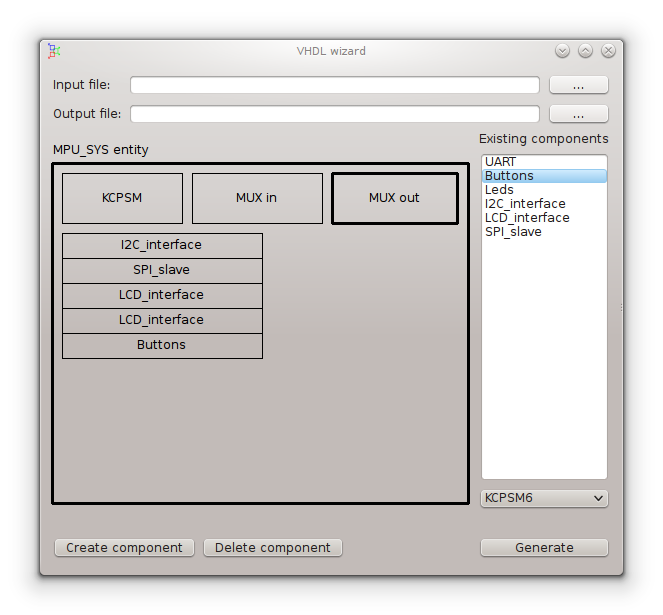
\includegraphics[width=.5\textwidth]{img/VHDL_wizard.png}
    \caption{VHDL Wizard}
\end{figure}

\subsubsection{Purpose of this tool}
    This tool is used for quicker connection between picoblaze and your vhdl design. It can help you, when you don't want spend too much time writing  peripheral logic for picoblaze
    and your VHDL components. It will automatically take PORT symbols from your assembler file and generates appropriate constants and input/output multiplexers. Final product of
    this program is one ENTITY containing your custom components, port constants, all necessary signals/constants and declaration of KCPSM design. In case somehow change your design, you
    can just click generate again and your vhdl file will adjust to new or edited values.  

\subsubsection{Main window}
    \begin{description}
        \item [Input file]
            VHDL wizard reads the symbol table file and extracts all symbols declared with PORT, PORTIN and PORTOUT directives. Select path to your .stbl(symbol table) file generated after the compilation of you assembler source code. Note, make sure you
            have generation of the file allowed (Project->Configure->Compiler->Options->Symbol table checked).
        \item [Output file]
            Select path for your generated VHDL template.
        \item [MPU\_SYS entity]
            General look to your template entity. Every box symbolizes vhdl component. There are always three default boxes. KCPSM component, Input demux.
            and output mux. You can click to every one of them for detail info. When you create or add some custom component, it will show
            up here. 
        \item [Existing components]
            This list contains all your previously defined components. Let's say you have an UART receiver in your design. You will then create your custom component named UART
            and define his ports and generic attributes. It will appear here and you can add it to your entity at any time. 
        \item [KCPSM combobox]
            You can select KCPSM version of your picoblaze design. It will change the declaration and instantiation of picoblaze in generated vhdl file. KCPSM6 is selected
            by default.
        \item [Create component button]
            This button will open create component dialog where you can define your new component. See the next section "Create component dialog".
        \item [Delete component button]
            This button will remove one component from your MPU\_SYS entity. 
        \item [Generate]
            If you have your input and output file selected. This button will trigger generation of VHDL template.
    \end{description}

\subsubsection{Create component dialog}
    You can define your custom component and add it to the generated entity or save it for later usage. You can \textbf{remove} or \textbf{edit} existing components by
    right-clicking them in the field "Existing components".
    
\begin{figure}[h]
    \centering
    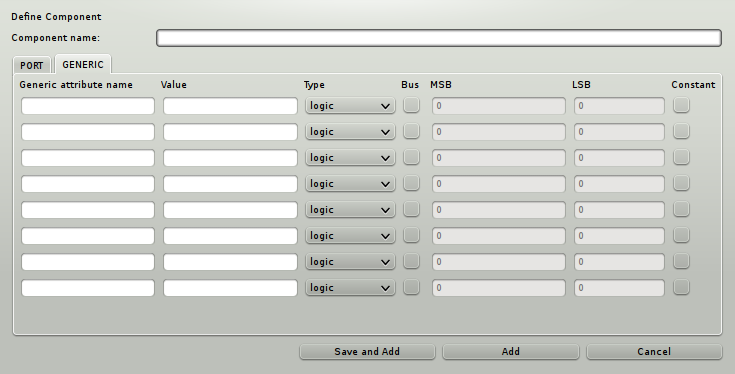
\includegraphics[width=.7\textwidth]{img/VHDL_create_generic.png}
    \caption{Custom component generic parameters}
\end{figure}

\begin{figure}[h]
    \centering
    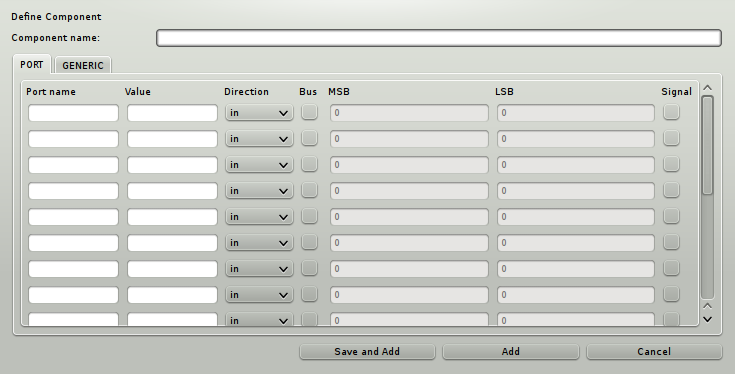
\includegraphics[width=.7\textwidth]{img/VHDL_create_component.png}
    \caption{VHDL port parameters}
\end{figure}

    \begin{description}
        \item [Component name]
            Name of your custom component.
        \item [Tab port and generic]
            Port tab lets you define component ports.
        \item [Port name/ Generic name]
            Name of evvery port or generic attribute. Names (or identifiers) may consist of letters, numbers and underscore.
        \item [Value]
            You can set the initial value. Leaving this field empty means no initial value is needed.
        \item [Direction/Type]
            Direction in port tab can be IN,OUT or INOUT. In generic tab, you define type of your generic attribute. Logic means zero or one. Logic vector is a bus, defined with MSB and LSB numbers.
            Integer can be number defined from range -2147483648 to +2147483647. Positive is RANGE 1 TO integer’HIGH. Natural is in RANGE 0 TO integer’HIGH.
        \item [Bus check-box]
            Telling generator, that this port is bus. Checking this will enable MSB(most significant bit) and LSB(least significant bit) field, which represents width of your bus.
            This check box in generic tab makes sense only for logic vector type of attribute.
        \item [Signal/Constant check-box]
            If checked, generator will insert this port or generic attribute declared as signal or constant in VHDL template.
        \item [Save and add button]
            Component will be added to MPU\_SYS entity and saved for later usage. Component name will appear in list "Existing components" and can be edited or added to current entity any time.
        \item [Add button]
            This button will add component to the current entity only once.
        \item [Generate]
            If you have your input and output file selected. This button will trigger generation of VHDL template.\\
    \end{description}
    